\documentclass[a4paper, 11pt, titlepage]{jsarticle}
\usepackage[dvipdfmx]{graphicx}
\usepackage{listings}
\usepackage{amsmath}
\usepackage{url}


\title{知能情報実験III(データマイニング班)\\指紋認証の分析と改善}
\author{185710A, 185714C, 185745C, 185752F, 185763B}
\date{提出日:2021年2月x日}
\begin{document}
\maketitle
\tableofcontents
\clearpage


\section{はじめに}
データマイニングとはデータの中に埋め込まれている有用な知識を発掘することである。別の言い方では、データマイニングは、より良い意思決定をするために履歴データをうまく使って一般的な規則性を発見しよとする研究分野である。今回私たちのグループ3では、機会学習の基本的な考え方を実装、体験を通して学んだ。そしてその応用として、既存に存在する指紋データを使った指紋認証のプログラムの分析から、結果の改善と精度向上を目指し、その結果を可視化し、考察したことについて考察する。

\subsection{Convolutional Neural Network:CNN}
Convolutional Neural Network (これよりCNNと呼ぶ)は畳み込みニューラルネットワークという意味であり、機械学習で画像の深層学習といえばCNNであるというほどよく使われている識別手法である。これは、ニューラルネットワークに畳み込みという操作を導入したものである。CNNについて、簡単な手順を記述する。まず手順1として、\textbf{画像から特徴を抽出}する。フィルタを使い、入力層データの中で位置を変えながらスキャンした部分のデータと、フィルター自身の持つデータとの差異を畳み込みの結果として畳み込みそうに書き込んだものを特徴量といい、入力層の全データをスキャンしてできた畳み込み結果の値の集まりを特徴マップという。複数のフィルタを用意することで、入力層のデータ特徴を捉えやすくしている。下の図は用意した複数フィルタのうち、一つが完全に入力層のデータの一部と同じであることを示す。

\begin{figure}[h]
  \centering
  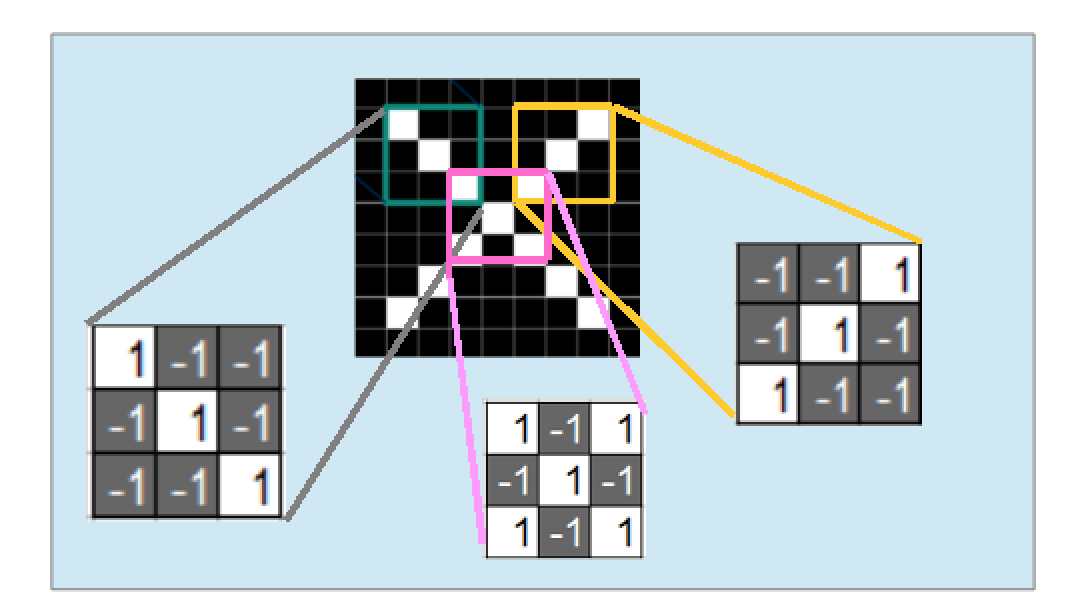
\includegraphics[scale=0.4]{cnn1.png}
  \caption{CNN解説手順1}
  \label{cnn}
\end{figure}


手順2として、\textbf{画像を畳み込み}する。入力層のデータをフィルターのデータとピクセル毎に比較することで、畳み込み層にその類似度(特徴量)を書き込む。下記の図はフィルタを利用して特徴量を抽出し、特徴マップを作成した例である。

\begin{figure}[h]
  \centering
  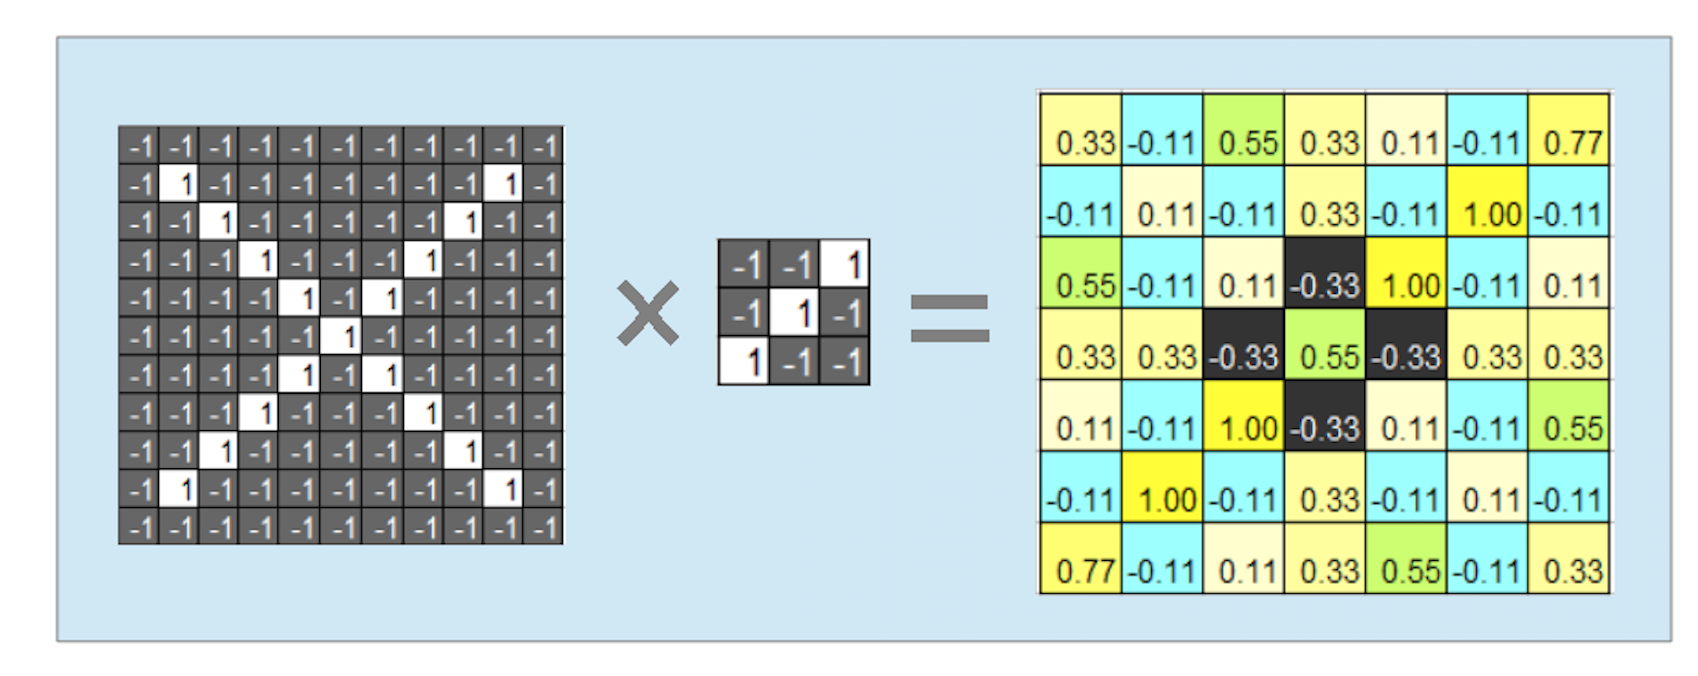
\includegraphics[scale=0.3]{cnn2.png}
  \caption{CNN解説手順2}
  \label{cnn}
\end{figure}

手順3として、\textbf{画像をプーリング}する。畳み込みの層の情報はプーリング層で集約する。出力に関しては、プーリング層のユニット全てと全結合し、計算結果を利用して、フィルタ、重み、バイアスを更新していく。

\begin{figure}[h]
  \centering
  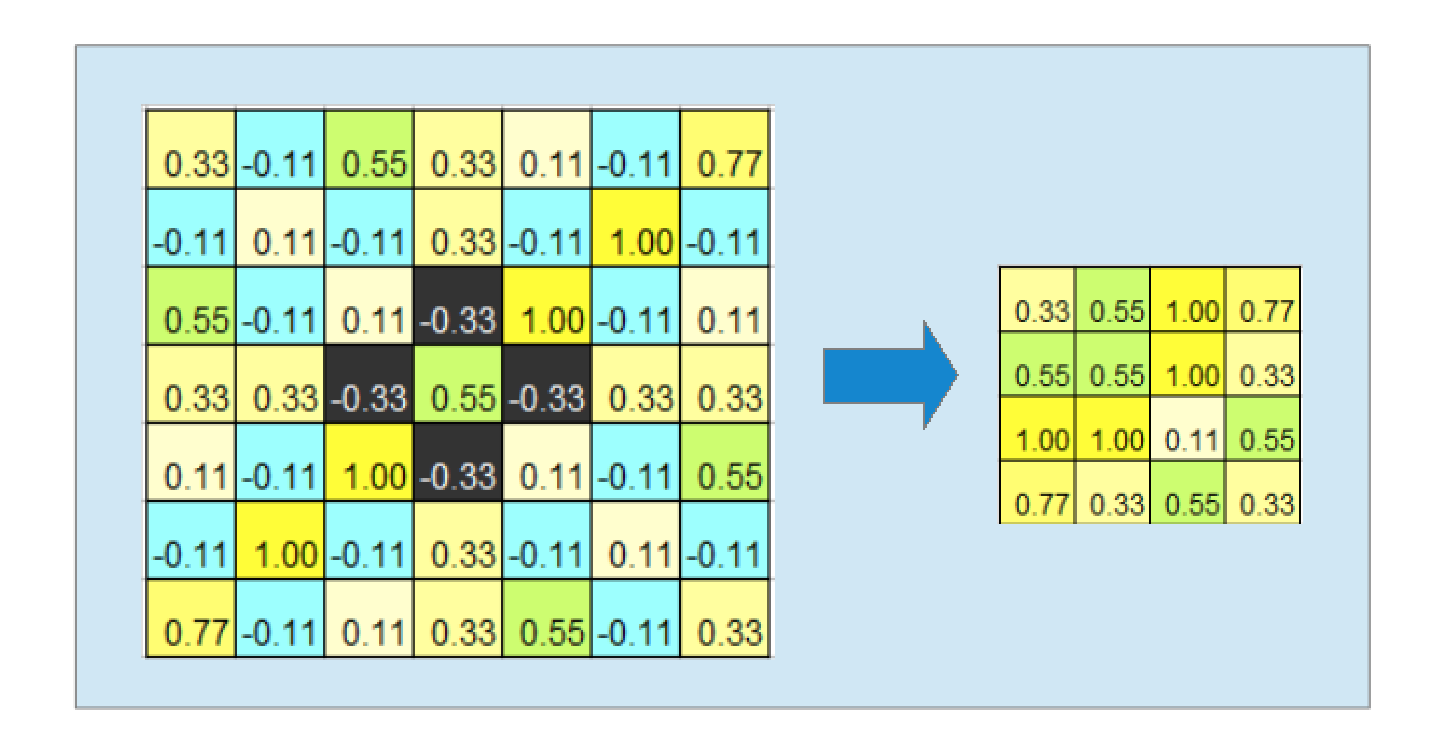
\includegraphics[scale=0.4]{cnn3.png}
  \caption{CNN解説手順3}
  \label{cnn}
\end{figure}


\subsection{実験の目的}


\subsection{テーマ指紋認証とは}
本グループでは、授業の中でデータマイニングについて学び、それらの応用実験として、画像認識について分析しようと考えた。そして、データマイニングを行う識別手としてCNNに目をつけ、データの分類ラベルがはっきりしており、複雑である指紋認証の分析、精度改善を行うこととなった。CNNは畳み込み処理を利用したニューラルネットワークであり、どのくらい畳み込み処理を行うのか、どのくらいニューラルネットワークを深くするのかは定義されていない。

(例)
本グループでは**における**することを対象問題として設定した。
**とは\cite{theme1}によると〜〜〜であり、**を**することで**に寄与する。
また\cite{theme2}によると〜〜〜とも述べられており、



\section{実験方法}
実験手順を過去形で述べよう。日誌のように時系列ではなく、成果物として報告する最終版を再現するための実験手順で良い。
第三者が再現するために必要な手順であることが重要だ。
また、列挙した項目毎に具体的な内容をsubsectionで述べよう。

(あくまでも例です)
\begin{enumerate}
 \item 実験目的
 \item 実験計画
 \item データセット構築
 \item モデルの選定
 \item パラメータ調整
\end{enumerate}

\subsection{実験目的}
実験を通して明らかにしたいこと、確認したいこと、検証したいことを述べよう。

\subsection{データセット構築}
既にどこかで公開されているデータセットをダウンロードして利用したのならば、そのURLを掲載する程度で構いません。
独自構築した場合にはその構築方法を述べよう。

\subsection{モデル選定}
どのようなモデルやアルゴリズムを利用したのか、何故それを選んだのか述べよう。

\subsection{パラメータ調整}
手動調整が必要なパラメータについて、どのように調整したのか述べよう。


\section{実験結果}
事実として得られた結果を示そう。
なお、以下の点に留意すること。

\begin{itemize}
 \item 「思う」「思われる」のような主観ではなく、客観的事実を述べること。
 \item 図表には適切なキャプションを付けること。
 \item 挿入した図表について、本文中でその読み方を述べること。その際にはlabel, refにより相互参照すること。
 \item レポートにおけるグラフの作成においては、以下の点に注意する。
 \begin{itemize}
 	\item 軸目盛および軸ラベルに関する注意事項
 	\begin{itemize}
 		\item 必ず軸ラベルを表示する
 		\item 軸に単位がある場合には、ラベルに単位を付記する
 		\item 軸目盛は適切な感覚で表示する
 		\item 軸目盛は述べたい内容に応じて線形スケールとlogスケールを使い分ける
 		\item 印刷時に明瞭に読むことができるサイズで表示する
 	\end{itemize}
 	\item 線・点・ポイントおよび凡例に関する注意事項
 	\begin{itemize}
 		\item 線・点・ポイントは、印刷時に明瞭に識別できる太さやサイズで表示する
 		\item 1つのグラフに複数にデータを表示する際には、データごとに異なる線種、線の太さ、ポイント形状などを使用する
 		\item モノクロ印刷でも識別できるように線・点・ポイントを使用することが望ましい
 		\item 凡例は線・点・ポイントに重ならないように注意する
 	\end{itemize}
 \end{itemize}
\end{itemize}

\section{考察}
実験課題への取り組みを通し、実験の意義、実験からわかったこと、今後の展望などを述べる。
失敗やつまづきがあれば、それらについての失敗分析を含めると良い。

\section{意図していた実験計画との違い}
グループワークとして2ヶ月程度の時間が用意されていた。
ガントチャート\ref{ganttchart}等、何かしら工夫して全体の計画を述べよう。
これらの期間をどのように使おうとし、実際どうだったのかについて自己評価(振り返り)してみよう。
大きなズレがある場合それは何故起きたのか、どうやればそのギャップを縮められそうか検討してみよう。

\section{まとめ}
データマイニング班の達成目標を振り返り、選んだテーマに対する機械学習の適用を通して得られた知見や学んだことをまとめよう。
また今後やるべきことや後進に伝えたいこと等あれば自由に述べよう。

\begin{thebibliography}{n}
  \bibitem{kanazawa}レポート作成の手引き レポートの基本的形式に関するガイド, \url{https://www.kanazawa-u.ac.jp/wp-content/uploads/2015/01/tebiki2.pdf}, 2020/07/02.
	\bibitem{theme1}テーマ出典, 書籍or特定の記事or webpage, webpageの場合は参照日も記そう, 2020/07/02.
	\bibitem{theme2}テーマ出典2, 出典は半角,.で書こう.
	\bibitem{ganttchart}ガントチャート, \url{https://ja.wikipedia.org/wiki/ガントチャート}, 2020/07/02.
\end{thebibliography}
\end{document}
